\documentclass{article}
\usepackage{hyperref}
\usepackage{amsmath}
\usepackage{amssymb}
\usepackage{pgfplots}
\usepackage{float}
\usepackage{todonotes}
\usepackage{tikz}

\renewcommand{\Re}{\mathbb{R}}
\newcommand{\Li}{\mathcal{L}}
\newcommand{\Ex}{\mathbb{E}}
\renewcommand{\Pr}{\mathbb{P}}
\newcommand{\Hy}{\mathcal{H}}

\newcommand\bigO[1]{
    \ensuremath{\mathcal{O}\left(#1\right)}
    }

\newcommand{\sigmoidPlot}{
    
    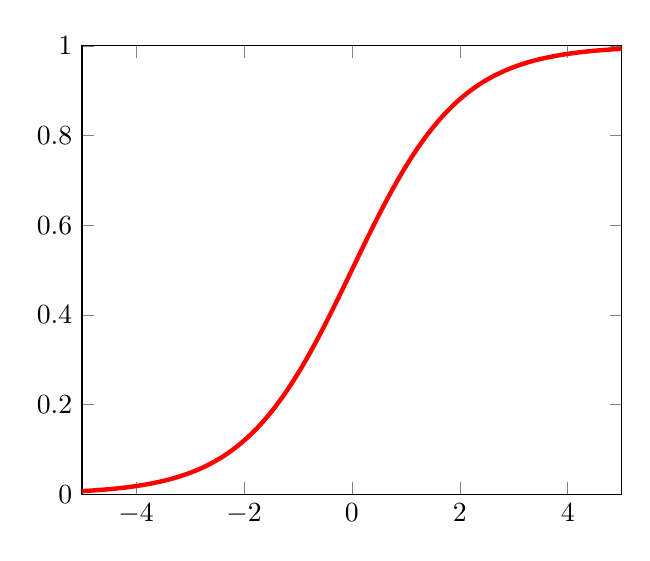
\begin{tikzpicture}
        \begin{axis}[xmin=-5, xmax=5, ymin=0, ymax=1, samples=150]
        \addplot[red, ultra thick] {1/(1+exp(-x))};
        \end{axis}
    \end{tikzpicture}
    
    }

\usetikzlibrary{positioning, calc}
\usetikzlibrary{arrows.meta}

\tikzstyle{circlebox}=[circle,thick,draw=black!75,minimum size=8mm]
\tikzstyle{inputnode}=[circlebox, draw=blue!75]
\tikzstyle{hiddennode}=[circlebox, draw=orange!75]
\tikzstyle{outputnode}=[circlebox, draw=orange!75]
\tikzstyle{simplebox}=[rectangle,thick,draw=black!75,
fill=black!20,minimum size=4mm]
\tikzstyle{textbox}=[rectangle,thick,minimum size=4mm,draw=black!0,
fill=black!0]
\tikzstyle{halfvdistance}=[yshift=-0.7cm]
\tikzstyle{abovebetween}=[xshift=-2.7mm]
\tikzstyle{edgepath} = [-Latex,->,shorten >=1pt,-stealth,semithick, rounded 
corners=5pt]

\def \nodedv {0.735cm}
\def \nodedh {0.65cm}

\tikzset{
    between/.style args={#1 and #2}{
        at = ($(#1)!0.5!(#2)$)
    }
}

\begin{document}
    \section{Subjects}
    \begin{itemize}
        \item Basic algorithms and applications
        \item Building models and selecting model parameters
    \end{itemize}
    
    \section{Notes}
    
    \subsection{Motivation for HMM}
    
    Our predictions are based on models of observed data, a simple model is 
    that observations are assumed to be independent and identically distributed.
    
    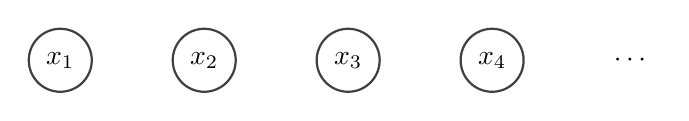
\begin{tikzpicture}
    \node[circlebox] (x1) {$x_1$};
    \node[circlebox, right=of x1] (x2) {$x_2$};
    \node[circlebox, right=of x2] (x3) {$x_3$};
    \node[circlebox, right=of x3] (x4) {$x_4$};
    \node[textbox, right=of x4] (dots) {$\cdots$};
    \end{tikzpicture}
    
    But this assumption is not always the best, an example is measurements of 
    weather patterns, daily value of stocks etc. In these cases, a model that 
    shows how each observation depends on the previous observations might be 
    better.
    
    \begin{equation*}
        p(x_n|x_1,\dots.x_{n-1})=p(x_n|x_{n-1})
    \end{equation*}
     This can be depicted as:
    
    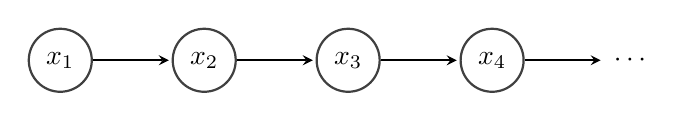
\begin{tikzpicture}
    \node[circlebox] (x1) {$x_1$};
    \node[circlebox, right=of x1] (x2) {$x_2$};
    \node[circlebox, right=of x2] (x3) {$x_3$};
    \node[circlebox, right=of x3] (x4) {$x_4$};
    \node[textbox, right=of x4] (dots) {$\cdots$};
    
    \path[edgepath]
        (x1) edge node {} (x2)
        (x2) edge node {} (x3)
        (x3) edge node {} (x4)
        (x4) edge node {} (dots);
    \end{tikzpicture}
    
    This chain of observations is a 1st-order Markov chain. The joint 
    probability of observing some sequence of $N$ observations is then:
    \begin{equation*}
        p(x_1,\dots,x_N)=\prod_{n=1}^{N}p(x_n|x_1,\dots,x_{n-1}) = 
        p(x_1)\prod_{n=2}^{N}p(x_n|x_{n-1})
    \end{equation*}
    
    For example, suppose the weather has two states, sun and rain. It might be 
    that if the weather is sunny, then with probability $\frac{6}{7}$ it will 
    stay sunny and $\frac{1}{7}$ it will start to rain however if it's already 
    raining then the probability that it will keep raining is not $\frac{1}{7}$ 
    but instead it might be $\frac{2}{3}$, with just $\frac{1}{3}$ chance it 
    will turn sunny. So the probability of some observation, depends on the 
    last observation, or ``what state are we currently in''.
    
    Now suppose the state that influences the weather is not necessarily what 
    the last observation was, but rather some other state that is hidden to us? 
    For example wether there is a high or low pressure. If the hidden variables 
    are discrete and form a Markov chain, then we can model it as a hidden 
    Markov model (HMM).
    
    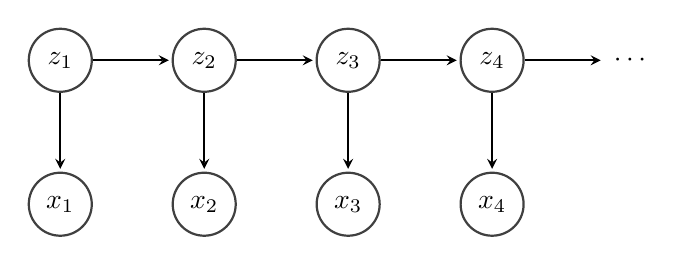
\begin{tikzpicture}
    \node[circlebox] (z1) {$z_1$};
    \node[circlebox, right=of z1] (z2) {$z_2$};
    \node[circlebox, right=of z2] (z3) {$z_3$};
    \node[circlebox, right=of z3] (z4) {$z_4$};
    \node[textbox, right=of z4] (dots) {$\cdots$};
    \node[circlebox, below=of z1] (x1) {$x_1$};
    \node[circlebox, below=of z2] (x2) {$x_2$};
    \node[circlebox, below=of z3] (x3) {$x_3$};
    \node[circlebox, below=of z4] (x4) {$x_4$};
    
    \path[edgepath]
    (z1) edge node {} (z2)
    (z2) edge node {} (z3)
    (z3) edge node {} (z4)
    (z4) edge node {} (dots)
    (z1) edge node {} (x1)
    (z2) edge node {} (x2)
    (z3) edge node {} (x3)
    (z4) edge node {} (x4);
    \end{tikzpicture}
    
    The joint distribution is then:
    
    \begin{equation*}
        p(x_1,\dots,x_N,\,z_1,\dots,z_N) = 
        p(z_1)\left[\prod_{n=2}^{N}p(z_n|z_{n-1})\right] 
        \prod_{n=1}^{N}p(x_n|z_n)
    \end{equation*}
    Then here we can see that 
    $p(z_1)\left[\prod_{n=2}^{N}p(z_n|z_{n-1})\right]$ models the probability 
    that we are in state $z_n$ given states $z_1,\dots,z_{n-1}$. And the 
    probability $\prod_{n=1}^{N}p(x_n|z_n)$ is the probability that, given we 
    are in some state $z_n$, we make the observation $x_n$.
    
    \subsubsection{Modeling transmission probabilities}
    Notation: we write the hidden variables as positional vectors, i.e. if 
    $z_n=(0,0,1)$ then the model in step $n$ is in state $k=3$.
    
    Given that the hidden variables had to be discrete in order to model them 
    with a HMM, we know that the have $K$ states. Since we know that the amount 
    of states are limited, we can model the transmission probabilities as a 
    $K\times K$ table called $A$. And we can describe the initial state given 
    by the probability distribution $p(z_1)$ as a $K$ vector $\pi$. We can 
    describe this formally as:
    
    \begin{equation*}
        A_{jk} = p(z_{nk}=1|z_{n-1,j}=1), \quad \pi_k = p(z_{1k}=1)
    \end{equation*}
    We then have that:
    \begin{equation*}
        \sum_{k}A_{jk}=1,\quad \sum_k \pi_k=1
    \end{equation*}
    We can then write the math cleverly like this:
    \begin{equation*}
        p(z_n|z_{n-1},A)=\prod_{k=1}^{K}\prod_{j=1}^{K}A_{jk}^{z_{n-1,j}z_{nk}},
        \quad p(z_1|\pi)=\prod_{k=1}^{K}\pi_k^{z_{1k}}
    \end{equation*}
    Now, this may look confusing. but remember that the hidden variables are 
    positional vectors. That is: 
    \begin{equation*}
        z_1=\begin{pmatrix}
            0\\
            \vdots\\
            0\\
            1\\
            0\\
            \vdots\\
            0
        \end{pmatrix}
    \end{equation*}
    So when we say $\pi_k^{z_{1k}}$ then $z_{1k}$ will be equal to $0$ for all 
    entries except one where it is $1$. Thus we will have a product of $\pi_0^0 
    \cdots \pi_{i-1}^0 \cdot \pi_{i}^1 \cdot \pi_{i+1}^0 \cdots \pi_K^0$. So it 
    is really just a way of extracting a single value out of $\pi$ and $A$.
    
    \subsubsection{Modeling emission probabilities}
    Similar to the transmission probabilities, if we assume that the observed 
    values $x_n$ are discrete (e.g. $D$ different symbols), then the emission 
    probabilities $\phi$ can be modeled as a $K\times D$ table of 
    probabilities, which for each state $K$ specifies the probability of 
    observing some symbol.
    
    \begin{equation*}
        p(x_n|z_n,\phi)=\prod_{k=1}^K p(x_n|\phi_k)^{z_{nk}}
        = \prod_{k=1}^K \prod_{d=1}^{D} \phi_{kd}^{x_{nd},z_{nk}}
    \end{equation*}
    
    We then get the joint probability distribution of the HMM:
    
    \begin{equation*}
        p(X,Z|\Theta) = 
        p(z_1|\pi)\left[\prod_{n=2}^{N}p(z_n|z_{n-1},A)\right] 
        \prod_{n=1}^{N}p(x_n|z_n,\phi)
    \end{equation*}
    
    With our observables being: $X=\{x_1,\dots,x_N\}$ the latent states being:
    $Z=\{z_1,\dots,z_N\}$ and our model parameters: $\Theta=\{\pi, A, \phi\}$
    \\
    The matrix $A$ looks like this:\\
    \\
    \includegraphics[width=7cm]{Figures/trans_prob_A.pdf}
    
    Where: $A_{jk}=p(z_{nk}=1|z_{n-1,j}=1)=\text{ probability of going from $j$ 
    to $k$}$

    The matrix $\pi$ looks like this:\\
    \\
    \includegraphics[width=4cm]{Figures/init_prob_PI.pdf}
    
    Where: $\pi_k=p(z_{nk}=1)$.
    
    The matrix $\phi$ looks like this:\\
    \\
    \includegraphics[width=7cm]{Figures/emis_prob_PHI.pdf}
    
    Where: $\phi_{kd}=p(x_{nd}=1|z_{nk}=1)=$ probability of seeing observation 
    $d$ in state $k$.
    
    \subsubsection{HMM as a generative model}
    There are two goals we might have when we are using HMMs, first is to 
    determine the likelihood of a sequence of observations. The second is to 
    find a plausible underlying explanation (or decoding) of a sequence of 
    observations.
    
    Determining the likelihood of a sequence of observations are computed like 
    this:
    \begin{equation*}
        p(X|\Theta) = \sum_Z p(X,Z|\Theta)
    \end{equation*}
    This sum has $K^N$ terms, but it turns out that it can actually be computed 
    in \bigO{K^2N} time. But let's look at decoding first.
    
    \subsubsection{Decoding using HMMs}
    Given a HMM $\Theta$ and a sequence of observations $X=x_1,\dots,x_N$, then 
    find a plausible explanation $Z^*=z^*_1,\dots,z^*_N$ of values of the 
    hidden variable.
    We will look at two types of decoding here, Viterbi deconding and Posterior 
    decoding.
    
    \begin{description}
        \item[Viterbi decoding] $Z^*$ is the overall most likely explanation of 
        $X$:
        \begin{equation*}
            Z^* = \arg\max_Z p(X,Z|\Theta)
        \end{equation*}
        \item[Posterior decoding] $z^*_n$ is the most likely state to be in the 
        $n$'th step:
        \begin{equation*}
            z^*_n=\arg\max_{z_n} p(z_n|x_1,\dots,x_N)
        \end{equation*}
    \end{description}
    
    \subsubsection{Viterbi decoding}
    Given $X$, find $Z^*$ such that: $Z^*=\arg\max_Z p(X,Z|\Theta)$
    
    We can write the probability of $X$ given the optimal explanation $Z^*$ as 
    follows:
    
    \begin{align*}
        p(X,Z^*) &= \max_Z p(X,Z)\\
            &= \max_{z_1,\dots,z_N} p(x_1,\dots,x_N,\, z_1,\dots,z_N)\\
            &= \max_{z_N}\max_{z_1,\dots,z_{N-1}} p(x_1,\dots,x_N, \, z_1, 
            \dots, z_N)\\
            &= \max_{z_N}\omega(z_N)\\
            z^*_N &= \arg\max_{z_N} \omega(z_N)
    \end{align*}
    
    Here, $\omega(z_n)=\max\limits_{z_1,\dots,z_{n-1}} 
    p(x_1,\dots,x_n,\,z_1,\dots,z_n)$ is the probability of the most likely 
    sequence of states $z_1,\dots,z_n$ ending in $z_n$ generating the 
    observations $x_1,\dots,x_n$.
    
    We can expand $\omega(z_n)$ as follows:
    \begin{align*}
        \omega(z_n)&=\max_{z_1,\dots,z_{n-1}}p(x_1,\dots,x_n,\,z_1,\dots,z_n)\\
            &=\max_{z_1,\dots,z_{n-1}} p(z_1) \prod_{i=2}^n p(z_i|z_{i-1}) 
            \prod_{i=1}^{n}p(x_i|z_i)\\
            &=p(x_n|z_n)\max_{z_1,\dots,z_{n-1}} 
            p(z_1)\prod_{i=2}^{n}p(z_i|z_{i-1}) \prod_{i=1}^{n-1}p(x_i|z_i)\\
            &\vdots\\
            &=p(x_n|z_n) \max_{z_{n-1}} p(z_n|z_{n-1})\omega(z_{n-1})
    \end{align*}
    So the $\omega$ is recursive, we can sum up $\omega$ as follows:
    \begin{description}
        \item[Recursion]
        \begin{equation*}
            \omega(z_n)=p(x_n|z_n) \max_{z_{n-1}} \omega(z_{n-1})p(z_n|z_{n-1})
        \end{equation*}
        \item[Basis]
        \begin{equation*}
            \omega(z_1)=p(x_1,z_1)=p(z_1)p(x_1|z_1)
        \end{equation*}
    \end{description}
    We can describe the $\omega$ function as a $N\times K$ matrix, 
    $\omega[k][n]=\omega(z_n)$ if $z_n$ is state $k$, and construct it as 
    follows:
    \begin{enumerate}
        \item $\omega[k][n] = 0$
        \item if $p(x[n]|k) \neq 0:$
        \begin{enumerate}
            \item for $j=1$ to $K$
            \begin{enumerate}
                \item if $p(k|j) \neq 0$
                \begin{enumerate}
                    \item $\omega[k][n]=\max(\omega[k][n], p(x[n]|k) \cdot 
                    \omega[j][n-1] \cdot p(k|j)$
                \end{enumerate}
            \end{enumerate}
        \end{enumerate}
    \end{enumerate}
    We can then compute $\omega$ in \bigO{K^2N} time, using \bigO{KN} space. 
    Now that we have $\omega(z_n)$, which is the probability of the most likely 
    sequence of states, that ends in $z_n$, we can find $Z^*$ by backtracking :
    \begin{align*}
        z^*_N &= \arg\max_{z_N}\omega(z_N) = \arg\max_{z_N}\max_{z_{N-1}} 
        \left(p(x_N|z_N)\omega(z_{n-1})p(z_N|z_{N-1})\right)\\
        z^*_{N-1} &= 
        \arg\max_{z_{N-1}}\left(p(x_N|z^*_N)\omega(z_{N-1}p(z^*_N|z_{N-1})\right)\\
        z^*_{N-2} &= 
        \arg\max_{z_{N-2}}\left(p(x_{N-1}|z^*_{N-1})\omega(z_{N-2}p(z^*_{N-1}|z_{N-2})\right)\\
    \end{align*}
    So we obviously have all that we need, we can just backtrack as follows:
    \begin{enumerate}
        \item $z[1\dots N] = \text{undef}$
        \item $z[N]=\arg\max_k \omega[k][N]$
        \item $n=N-1$ to $1$:
        \begin{enumerate}
            \item 
            \begin{equation*}
                z[n]=\arg\max_k\left(p(x[n+1]|z[n+1]) \cdot \omega[k][n] \cdot 
                p(z[n+1]|k)\right)
            \end{equation*}
        \end{enumerate}
        \item print $z[1\dots N]$
    \end{enumerate}
    We can backtrack in time \bigO{KN} using space \bigO{KN} using $\omega$.
    
    We could also use ``posterior decoding'', but it only works if there is a 
    transition from any state to any other state. In other cases it might not 
    return syntactically correct results.
    
    \subsubsection{Computing the likelihood of a sequence of observations}
    Apart from the $\omega$ recursion, we have the forward and backward 
    algorithms:
    \begin{description}
        \item[Forward algorithm] Computes $\alpha(z_n)$ which is the joint 
        probability of observing $x_1,\dots,x_n$ and being in state $z_n$:
        \begin{equation*}
            \alpha(z_n)=p(x_1,\dots,x_n,z_n)
        \end{equation*}
        \item[Backward algorithm] Computes $\beta(z_n)$ which is the 
        conditional probability of observing $x_{n+1},\dots,x_N$ in the future, 
        assuming we are in state $z_n$
        \begin{equation*}
            \beta(z_n)=p(x_{n+1},\dots,x_N|z_n)
        \end{equation*}
    \end{description}
    Then, having $\alpha(z_n)$ and $\beta(z_n)$, we can get the likelihood of 
    the observations as:
    \begin{equation*}
        p(X)=\sum_{z_n}\alpha(z_n)\beta(z_n), \quad p(X)\sum_{z_N}\alpha(z_N)
    \end{equation*}
    We can compute $\alpha$ as:
    \begin{description}
        \item[Recursion]
        \begin{equation*}
            \alpha(z_n)=p(x_n|z_n) \sum_{z_{n-1}} \alpha(z_{n-1})p(z_n|z_{n-1})
        \end{equation*}
        \item[Basis]
        \begin{equation*}
            \alpha(z_1)=p(x_1,z_1)=p(z_1)p(x_1|z_1)
        \end{equation*}
    \end{description}
    And we can compute $\beta$ as:
    \begin{description}
        \item[Recursion]
        \begin{equation*}
        \beta(z_n)=\sum_{z_{n+1}} 
        \beta(z_{n+1})p(x_{n+1}|z_{n+1})p(z_{n+1}|z_{n})
        \end{equation*}
        \item[Basis]
        \begin{equation*}
        \beta(z_N)=1
        \end{equation*}
    \end{description}
    
    \subsubsection{Training HMMs}
    
\end{document}